\documentclass{article}
\usepackage[utf8]{inputenc}
\usepackage{amsmath,amssymb}
\usepackage{tikz}
\usetikzlibrary{arrows.meta, positioning, calc}

\tikzset{
    block/.style = {draw, rectangle, minimum height=0.9cm, minimum width=1.4cm, align=center, thick, fill=blue!5},
    sum/.style = {draw, circle, minimum size=6mm, thick, fill=gray!10},
    input/.style = {coordinate},
    output/.style = {coordinate},
    sfgarrow/.style={-{Latex[length=2.5mm,width=1.5mm]}, thick, draw=blue!80!black}
}

\begin{document}

\subsection*{Diagram Asli Sistem}
\begin{center}
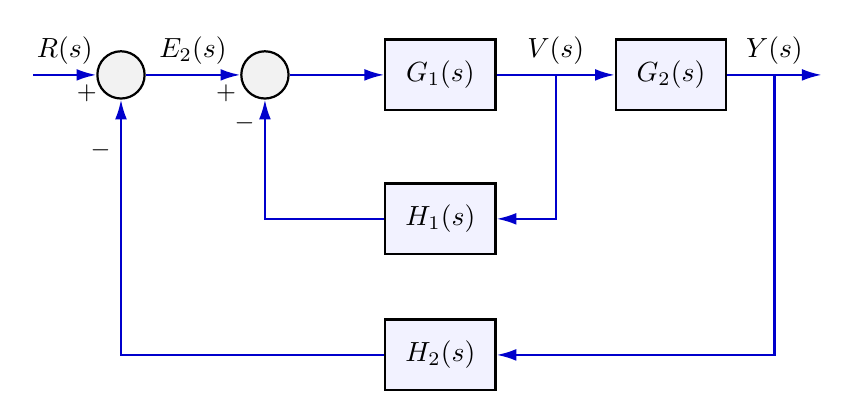
\begin{tikzpicture}[auto, >=Latex]
    \node [input] (input) {};
    \node [sum, right=0.8cm of input] (sum1) {};
    \node [sum, right=1.2cm of sum1] (sum2) {};
    \node [block, right=1.2cm of sum2] (g1) {$G_1(s)$};
    \node [block, right=1.5cm of g1] (g2) {$G_2(s)$};
    \node [output, right=1.2cm of g2] (output) {};
    
    \draw [sfgarrow] (input) -- node {$R(s)$} node[pos=0.85, below] {\small $+$} (sum1);
    \draw [sfgarrow] (sum1) -- node[above] {$E_2(s)$} node[pos=0.85, below] {\small $+$} (sum2);
    \draw [sfgarrow] (sum2) -- (g1);
    \draw [sfgarrow] (g1) -- node [name=v, above] {$V(s)$} (g2);
    \draw [sfgarrow] (g2) -- node [name=y, above] {$Y(s)$} (output);
    
    % Lup dalam H1
    \node [block, below=0.9cm of g1] (h1) {$H_1(s)$};
    \draw [sfgarrow] (v) |- (h1);
    \draw [sfgarrow] (h1) -| node[pos=0.9, left] {\small $-$} (sum2);
    
    % Lup luar H2
    \node [block, below=0.8cm of h1] (h2) {$H_2(s)$};
    \draw [sfgarrow] (y) |- (h2);
    \draw [sfgarrow] (h2) -| node[pos=0.9, left] {\small $-$} (sum1);
\end{tikzpicture}
\end{center}

\subsection*{Tahap 1: Isolasi Lup Bagian Dalam}
\begin{center}
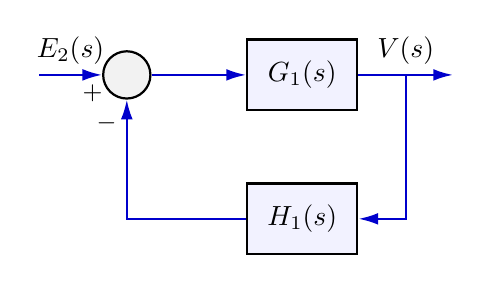
\begin{tikzpicture}[auto, >=Latex]
    \node [input] (in) {};
    \node [sum, right=0.8cm of in] (s2) {};
    \node [block, right=1.2cm of s2] (g1) {$G_1(s)$};
    \node [output, right=1.2cm of g1] (out) {};
    \node [block, below=0.9cm of g1] (h1) {$H_1(s)$};
    
    \draw [sfgarrow] (in) -- node {$E_2(s)$} node[pos=0.85, below] {\small $+$} (s2);
    \draw [sfgarrow] (s2) -- (g1);
    \draw [sfgarrow] (g1) -- node [name=v, above] {$V(s)$} (out);
    \draw [sfgarrow] (v) |- (h1);
    \draw [sfgarrow] (h1) -| node[pos=0.9, left] {\small $-$} (s2);
\end{tikzpicture}
\end{center}

\subsection*{Tahap 2: Substitusi Blok Ekuivalen $G_{in}(s)$}
\begin{center}
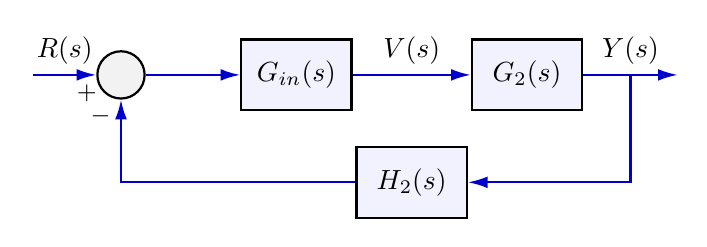
\begin{tikzpicture}[auto, >=Latex]
    \node [input] (input) {};
    \node [sum, right=0.8cm of input] (sum1) {};
    \node [block, right=1.2cm of sum1] (gin) {$G_{in}(s)$};
    \node [block, right=1.5cm of gin] (g2) {$G_2(s)$};
    \node [output, right=1.2cm of g2] (output) {};
    \node [block, below=0.9cm of $(gin)!0.5!(g2)$] (h2) {$H_2(s)$};
    
    \draw [sfgarrow] (input) -- node {$R(s)$} node[pos=0.85, below] {\small $+$} (sum1);
    \draw [sfgarrow] (sum1) -- (gin);
    \draw [sfgarrow] (gin) -- node [above] {$V(s)$} (g2);
    \draw [sfgarrow] (g2) -- node [name=y, above] {$Y(s)$} (output);
    \draw [sfgarrow] (y) |- (h2);
    \draw [sfgarrow] (h2) -| node[pos=0.9, left] {\small $-$} (sum1);
\end{tikzpicture}
\end{center}

\subsection*{Tahap 3: Penggabungan Blok Seri Maju $G_{fwd}(s)$}
\begin{center}
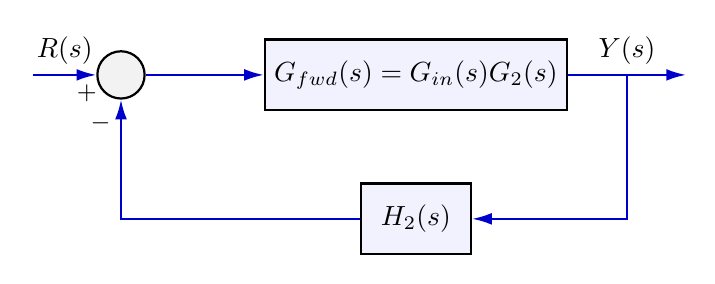
\begin{tikzpicture}[auto, >=Latex]
    \node [input] (input) {};
    \node [sum, right=0.8cm of input] (sum1) {};
    \node [block, right=1.5cm of sum1, minimum width=2.4cm] (gfwd) {$G_{fwd}(s) = G_{in}(s) G_2(s)$};
    \node [output, right=1.5cm of gfwd] (output) {};
    \node [block, below=0.9cm of gfwd] (h2) {$H_2(s)$};
    
    \draw [sfgarrow] (input) -- node {$R(s)$} node[pos=0.85, below] {\small $+$} (sum1);
    \draw [sfgarrow] (sum1) -- (gfwd);
    \draw [sfgarrow] (gfwd) -- node [name=y, above] {$Y(s)$} (output);
    \draw [sfgarrow] (y) |- (h2);
    \draw [sfgarrow] (h2) -| node[pos=0.9, left] {\small $-$} (sum1);
\end{tikzpicture}
\end{center}

\subsection*{Tahap 4: Blok Tunggal Lingkar Tertutup Total $T(s)$}
\begin{center}
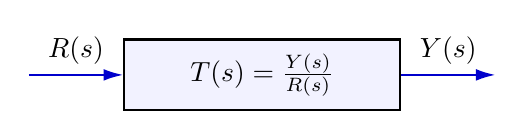
\begin{tikzpicture}[auto, >=Latex]
    \node [input] (input) {};
    \node [block, right=1.2cm of input, minimum width=3.5cm] (tot) {$T(s) = \frac{Y(s)}{R(s)}$};
    \node [output, right=1.2cm of tot] (output) {};
    
    \draw [sfgarrow] (input) -- node {$R(s)$} (tot);
    \draw [sfgarrow] (tot) -- node {$Y(s)$} (output);
\end{tikzpicture}
\end{center}

\end{document}
